% SciPy 最小二乘法
\pentry{Python 入门\upref{Python}}

\subsection{最小二乘拟合}
最小二乘法是一种数学优化技术.它通过最小化误差的平方和寻找数据的最佳函数匹配.利用最小二乘法可以简便地求得未知的数据,并使得这些求得的数据与实际数据之间误差的平方和为最小.

通常情况下最小二乘法是这样的:
给定一组数,假设是二维数据.$(x_1,y_1),(x_2,y_2),\cdots,(x_n,y_n)$ ,并且 $x,y$是相关的.假设满足方程,

\begin{equation}
y=f(x)
\end{equation}
但是这个方程我们是不知道具体什么样的.我们找到一个近似函数
\begin{equation}
y=g(x)
\end{equation}
y=g(x)

对于每一个点 $(x_i,y_i)$ 有 $y_i=g(x_i)+\epsilon_i$, $\epsilon_i$是残差. 那么总的残差平方和为
\begin{equation}
err=\sum_{i=1}^n(y_i-g(x_i)]^2
\end{equation}
那么我们就是要找到这样的$g(x)$使得如下公式中的$err$函数最小. 这种算法被称之为\textbf{最小二乘拟合}(Least-square fitting).

\verb|scipy|中的子函数库\verb|optimize|已经提供了实现最小二乘拟合算法的函数\verb|leastsq|.下面是用\verb|leastsq|进行数据拟合的一个例子:$y=A\sin(2\pi x+\theta)$.
\begin{lstlisting}[language=python]
import numpy as np
from scipy.optimize import leastsq
import pylab as plt
import matplotlib as mpl

mpl.rcParams["font.sans-serif"]=['kaiti']
mpl.rcParams['axes.unicode_minus']=False
def func(x, p):
 """
 数据拟合所用的函数: A*sin(2*pi*k*x + theta)
 """
 A, k, theta = p
 return A*np.sin(2*np.pi*k*x+theta)

def residuals(p, y, x):
  """
 实验数据x, y和拟合函数之间的差,p为拟合需要找到的系数
 """
  return y - func(x, p)

x = np.linspace(0, -2*np.pi, 100)
A, k, theta = 10, 0.34, np.pi/6 # 真实数据的函数参数
y0 = func(x, [A, k, theta]) # 真实数据
y1 = y0 + 2 * np.random.randn(len(x)) # 加入噪声之后的实验数据
p0 = [7, 0.2, 0] # 第一次猜测的函数拟合参数

 # 调用leastsq进行数据拟合
 # residuals为计算误差的函数
 # p0为拟合参数的初始值
 # args为需要拟合的实验数据
plsq = leastsq(residuals, p0, args=(y1, x))

print(u"真实参数:", [A, k, theta])
print(u"拟合参数", plsq[0]) # 实验数据拟合后的参数

plt.plot(x, y0, label=u"真实数据")
plt.plot(x, y1, label=u"\autoref{PyFit_fig1}带噪声的实验数据")
plt.plot(x, func(x, plsq[0]), label=u"拟合数据")
plt.xticks(fontsize=20)
plt.yticks(fontsize=20)
plt.legend()
plt.show()
\end{lstlisting}
结果图像如\autoref{PyFit_fig1}所示.
\begin{figure}[ht]
\centering
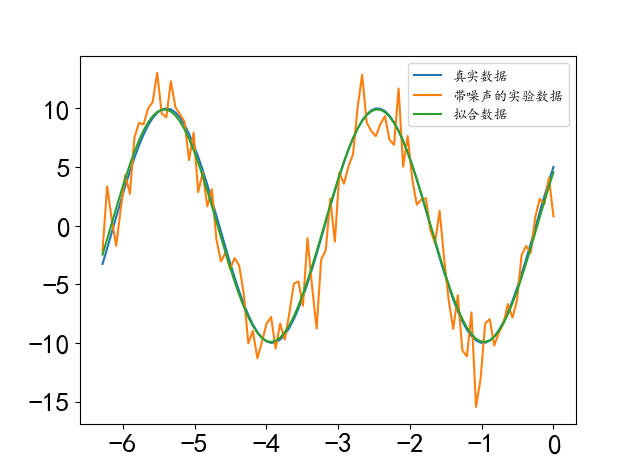
\includegraphics[width=8cm]{./figures/PyFit_1.png}
\caption{最小二乘法1} \label{PyFit_fig1}
\end{figure}

我们看到拟合参数虽然和真实参数完全不同,但是由于正弦函数具有周期性,实际上拟合参数得到的函数和真实参数对应的函数是一致的.

第二个例子:拟合$y=kx+b$.
\begin{lstlisting}[language=python]
# -*- coding: utf-8 -*-
import numpy as np
from scipy.optimize import leastsq
import pylab as plt
import matplotlib as mpl

mpl.rcParams["font.sans-serif"]=['kaiti']
mpl.rcParams['axes.unicode_minus']=False
def func(x, p):
 k,b = p
 return k*x+b

def residuals(p, y, x):
  """
 实验数据x, y和拟合函数之间的差,p为拟合需要找到的系数
 """
  return y - func(x, p)

x = np.linspace(0, -2*np.pi, 100)
k,b = 10, 5.0 # 真实数据的函数参数
y0 = func(x, [k,b]) # 真实数据
y1 = y0 + 2 * np.random.randn(len(x)) # 加入噪声之后的实验数据
p0 = [7, 0.2] # 第一次猜测的函数拟合参数

 # 调用leastsq进行数据拟合
 # residuals为计算误差的函数
 # p0为拟合参数的初始值
 # args为需要拟合的实验数据
plsq = leastsq(residuals, p0, args=(y1, x))

print(u"真实参数:", [k,b])
print(u"拟合参数", plsq[0]) # 实验数据拟合后的参数

plt.plot(x, y0, label=u"真实数据")
plt.plot(x, y1, label=u"带噪声的实验数据")
plt.plot(x, func(x, plsq[0]), label=u"拟合数据")
plt.xticks(fontsize=20)
plt.yticks(fontsize=20)
plt.legend()
plt.show()
\end{lstlisting}
拟合结果: 真实参数: \verb|[10, 5.0]|, 拟合参数\verb| [9.96688563 5.0180872 ]|. 图像如\autoref{PyFit_fig2}所示.
\begin{figure}[ht]
\centering
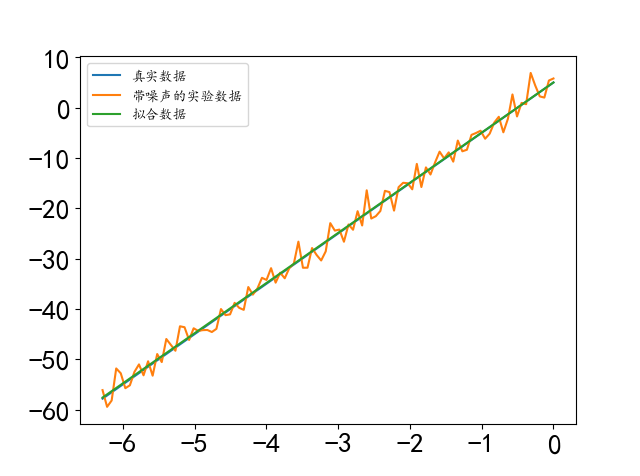
\includegraphics[width=8cm]{./figures/PyFit_2.png}
\caption{最小二乘法2} \label{PyFit_fig2}
\end{figure}


